\fenicschapter{FIAT: numerical construction of finite element basis functions}
              {FIAT: numerical construction of finite element basis functions}
              {FIAT: numerical construction of finite element basis functions}
              {Robert C. Kirby}
              {kirby-2}

The FIAT project~\citep{Kirby2004,Kirby2006} implements the
mathematical framework described in Chapter~\ref{chap:kirby-1} as a
Python package, working mainly in terms of numerical linear algebra.
Although an implementation in floating-point arithmetic presents some
challenges relative to symbolic computation, it can allow greater
efficiency in terms of work and memory usage, especially for high
order elements. To obtain efficiency in Python, the compute-intensive
operations are expressed in terms of numerical linear algebra and
performed using the widely distributed NumPy package. FIAT is one of
the first FEniCS projects, providing the basis function back-end for
FFC and enabling high-order $H^1$, $H(\mathrm{div})$ and
$H(\mathrm{curl})$ elements.

This chapter works in the context of a Ciarlet triple
$(T,\CiarletSpace,\mathcal{L})$ \citep{Ciarlet2002}, where $T$
is a fixed reference domain, typically a triangle or tetrahedron,
$\CiarletSpace$ is a finite-dimensional polynomial space, though perhaps
vector- or tensor-valued and not coincident with polynomials of some
fixed degree, and  $\mathcal{L} = \{ \ell_i \}_{i=1}^{|\CiarletSpace|}$ is
a set of linear functionals spanning $\CiarletSpace^\prime$.  Recalling
Chapter~\ref{chap:kirby-1}, the goal is first to enumerate a convenient
basis $\{ \phi_i \}_{i=1}^{|\CiarletSpace|}$ for $\CiarletSpace$ and
then to form a generalized Vandermonde system
\begin{equation}
  V A = I,
\end{equation}
where $V_{ij} = \ell_i( \phi_j)$.  Of course, forming this matrix
requires some calculations, and we will discuss this further in a
later section.  The columns of $A = V^{-1}$ store the expansion
coefficients of the nodal basis for $(T,\CiarletSpace,\mathcal{L})$ in
terms of some other basis $\{\psi_i\}$.

%------------------------------------------------------------------------------
\section{Prime basis: collapsed-coordinate polynomials}

High order polynomials in floating-point arithmetic require stable
evaluation algorithms.  FIAT uses the so-called collapsed-coordinate
polynomials~\citep{KarniadakisSherwin2005} on the triangle and tetrahedra.  Let
\(P^{\alpha,\beta}_i(x) \) denote the Jacobi polynomial of degree \( i
\) with weights \( \alpha \) and \( \beta \).  On the triangle \( T \)
with vertices \( (-1,-1) \), \((1,-1) \), \( (-1,1) \) and Cartesian
coordinates \( x\) and \( y \), the polynomials are of the form
\begin{equation}
  D^{p,q}( x,y ) = P^{0,0}_{p}(\eta_1)  \left( \frac{1-\eta_2}{2}
  \right)^p P^{2p+1,0}_q(\eta_2).
\end{equation}
Here, $\eta_1$ and $\eta_2$ are the Cartesian coordinates on
the biunit square, and the so-called collapsed-coordinate mapping
\[
\begin{split}
\eta_1 & = 2\left( \frac{1+x}{1-y} \right) - 1
\\
\eta_2 & = y
\end{split}
\]
maps from the triangle to the square.  The set $\{ D^{p,q}(x, y)
\}_{p,q \geqslant 0}^{p+q\leqslant n}$ forms a basis for polynomials
of degree~$n$).  Moreover, they are orthogonal in the $L^2(T)$ inner
product.  Recently, it has been shown that these polynomials may be
computed directly on the triangle without reference to the singular
mapping \citep{Kirby2009}.  This means that no special treatment of
the singular point is required, allowing use of standard automatic
differentiation techniques to compute derivatives.

The recurrences are obtained by rewriting the polynomials as
\[
D^{p,q}(x,y) = \chi^{p}(x,y) \psi^{p,q}(y),
\]
where \[
 \chi^{p}(x,y) = P^{0,0}_p(\eta_1) \left( \frac{1-\eta_2}{2}
\right)^p
\]
and
\[
\psi^{p,q}(y) = P^{2p+1,0}_q(\eta_2) = P^{2p+1,0}_q(y).
\]
This representation is not separable in \( \eta_1 \) and \( \eta_2
\), which may seem to be a drawback to readers familiar with the
usage of these polynomials in spectral methods.  However, they do
still admit sum-factorization techniques.  More importantly for
present purposes, each \( \chi^p \) is in fact a polynomial in \(
x \) and \( y \) and may be computed by recurrence.  \( \psi^{p,q}
\) is just a Jacobi polynomial in \( y \) and so has a well-known
three-term recurrence.  The recurrences derived in \citet{Kirby2009}
are presented in Algorithm~\ref{dubalg}, where, the coefficients \(
a_n^{\alpha,\beta},b_n^{\alpha,\beta},c_n^{\alpha,\beta} \) refer to
those used in the Jacobi polynomial recurrences.
\begin{equation}
\label{eq:recurcoeff}
\begin{split}
a^{\alpha,\beta}_n
  & = \frac{(2n + 1 + \alpha + \beta)(2n + 2 + \alpha + \beta)}
             {2(n+1)(n+1+\alpha+\beta)}
\\
b^{\alpha,\beta}_n
  & = \frac{(\alpha^2 -\beta^2)(2n+1+\alpha+\beta)}
             {2(n+1)(2n+\alpha+\beta)(n+1+\alpha+\beta)}\\
c^{\alpha,\beta}_n & = \frac{(n+\alpha)(n+\beta)(2n+2+\alpha+\beta)}
             {(n+1)(n+1+\alpha+\beta)(2n+\alpha+\beta)}.
\end{split}
\end{equation}
\begin{algorithm}
\caption{Compute all triangular orthogonal polynomials up to degree
  $d$ by recurrence}
\label{dubalg}
\begin{algorithmic}[1]
\State $D^{0,0}(x,y) := 1$
\State $D^{1,0}(x,y) := \frac{1+2x+y}{2}$
\For{$p \gets 1$, $d-1$}
\State $D^{p+1,0}(x,y) := \left( \frac{2p+1}{p+1} \right)
\left( \frac{1 + 2x + y}{2} \right) D^{p,0}(x,y)
- \left( \frac{p}{p+1} \right) \left( \frac{1-y}{2} \right)^2
D^{p-1,0}(x,y)$
\EndFor
\For{$p \gets 0,d-1$}
\State $D^{p,1}(x,y) := D^{p,0}(x,y) \left( \frac{1+2p+(3+2p) y}{2} \right)$
\EndFor
\For{$p \gets 0,d-1$}
\For{$q \gets 1,d-p-1$}
\State $D^{p,q+1}(x,y) :=
\left( a_{q}^{2p+1,0} y + b_q^{2p+1,0} \right) D^{p,q}(x,y)
- c_q^{2p+1,0} D^{p,q-1}(x,y)$
\EndFor
\EndFor
\end{algorithmic}
\end{algorithm}

\section{Representing polynomials and functionals}

Even using recurrence relations and NumPy vectorization for
arithmetic, further care is required to optimize performance.  In this
section, standard operations on polynomials will be translated into
vector operations, and then batches of such operations cast as matrix
multiplication.  This helps eliminate the interpretive overhead of Python
by moving numerical computation into optimized library routines,
since \texttt{numpy.dot} wraps level 3 BLAS and other functions such as
\texttt{numpy.svd} wrap relevant LAPACK routines.

Since polynomials and functionals over polynomials both form vector
spaces, it is natural to represent each of them as vectors representing
expansion coefficients in some basis.  So, let \( \{ \phi_i \} \) be the
Dubiner polynomials described above, where we have assumed
some linear indexing of the Dubiner polynomials.

Now, any \( p \in \CiarletSpace \) is written as a linear combination of the basis
functions \( \{ \phi_i \} \).  Introduce a mapping \( \mathcal{R} \) from
\( \CiarletSpace \) into \( \mathbb{R}^{|\CiarletSpace|} \) by taking the expansion coefficients
of \( p \) in terms of \( \{ \phi_i \} \).  That is,
\[
p = \mathcal{R}(p)_i \phi_i,
\]
where summation is implied over \( i \).

A polynomial \( p \) may then be evaluated at a point \( x \) as follows.
Let \( \Phi \) be the vector of basis functions tabulated at \( x \).
That is,
\begin{equation}
\label{eq:bigphi}
\Phi_i = \phi_i(x).
\end{equation}
Then, evaluating \( p \) follows by a simple dot product:
\begin{equation}
\label{eq:doteval}
p(x) = \mathcal{R}(p)_i \Phi_i.
\end{equation}

More generally in FIAT, a set of polynomials \( \{ p_i \} \) will need
to be evaluated simultaneously, such as evaluating all of the members
of a finite element basis.  The coefficients of the set of polynomials
may be stored in the rows of a matrix \( C \), so that
\[
C_{ij} = \mathcal{R}(p_i)_j.
\]
Tabulating this entire set of polynomials at a point \( x \) is simply
obtained by matrix-vector multiplication.  Let \( \Phi_i \) be as
in~(\ref{eq:bigphi}).  Then,
\[
p_i(x) = C_{ij} \Phi_j.
\]

The basis functions are typically needed at a set of points, such as
those of a quadrature rule.  Let \( \{ x_j \} \) now be a collection of
points in \( T \) and let
\[
  \Phi_{ij} = \phi_i(x_j),
\]
where the rows of \( \Phi \) run over the basis functions and the columns
over the collection of points.  As before, the set of polynomials may
be tabulated at all the points by
\[
p_i(x_j) = C_{ik} \Phi_{kj},
\]
which is just the matrix product \( C \Phi \) and may be efficiently
carried out by a library operation, such as the \texttt{numpy.dot}
wrapper to level~3 BLAS.

Finite element computation also requires the evaluation of derivatives
of polynomials.  In a symbolic context, differentiation presents no
particular difficulty, but working in a numerical context requires some
special care.

For some differential operator \( \partial \), the derivatives \(
\partial \phi_i \) are computed at a point \( x \), any polynomial \(
p = \mathcal{R}(p)_i \phi_i \) may be differentiated at \( x \) by
\[
\partial p(x) = \mathcal{R}(p)_i (\partial \phi_i),
\]
which is exactly analogous to~(\ref{eq:doteval}).  By analogy, sets of
polynomials may be differentiated at sets of points just like evaluation.

The formulae in Algorithm~\ref{dubalg} and their tetrahedral counterpart
are fairly easy to differentiate, but derivatives may also be obtained
through automatic differentiation.  Some experimental support for
this using the AD tools in Scientific Python has been developed in an
unreleased version of FIAT.

The released version of FIAT currently evaluates derivatives in terms
of linear operators, which allows the coordinate singularity in the
standard recurrence relations to be avoided.  For each Cartesian partial
derivative \( \frac{\partial}{\partial x_k} \), a matrix \( \partial^k \)
is calculated such that
\[
\mathcal{R}\left(\frac{\partial p}{\partial x_k}\right)_i
= \partial^k_{ij} \mathcal{R}(p)_j.
\]
Then, derivatives of sets of polynomials may be tabulated by
premultiplying the coefficient matrix \( C \) with such a \( \partial^k
\) matrix.  These matrices are constructed by tabulating the partial
derivatives of the Dubiner bases at a lattice of points and then
multiplying by a Vandermonde-type matrix that converts the lattice point
values to the expansion coefficients back in the Dubiner basis.

This paradigm may also be extended to vector- and tensor-valued
polynomials, making use of the multidimensional arrays implemented in
NumPy. Let \( P \) be a space of scalar-valued polynomials and
\( m > 0 \) an integer.  Then, a member of \( [P]^m \), a vector with \(
m \) components in \( P \), may be represented as a two-dimensional array.
Let \( p \in [P]^m \) and \( p^j \) be the \( j^\mathrm{th} \) component
of \( p \).  Then \( p^j = \mathcal{R}(p)_{jk} \phi_k \), so that \(
\mathcal{R}(p)_{jk} \) is the coefficient of \( \phi_k \) for \( p^j \).

The previous discussion of tabulating collections of functions at
collections of points is naturally extended to this context.  If \( \{ p_i
\} \) is a set of members of \( [P]^m \), then their coefficients may be
stored in an array \( C_{ijk} \), where \( C_i \) is the two-dimensional
array \( \mathcal{R}(p)_{jk} \) of coefficients for \( p_i \).  As before,
\( \Phi_{ij} = \phi_i(x_j) \) contains the values of the basis functions at a set
of points.  Then, the \( j^\mathrm{th} \) component of \( p \) at the
point \( x_k \) is naturally given by a three-dimensional array
\[
p_i(x_k)^j = C_{ijl} \phi_{lk}.
\]
If \( C_{ijl} \) is stored contiguously in generalized row-major format,
this is just a matrix product and no data motion is required to
use a library call.

Returning for the moment to scalar-valued polynomials, linear functionals
may also be represented as Euclidean vectors.  Let \( \ell: P \rightarrow
\mathbb{R} \) be a linear functional.  Then, for any \( p \in P \),
\[
\ell( p ) = \ell( \mathcal{R}(p)_i \phi_i )
= \mathcal{R}(p)_i \ell( \phi_i ),
\]
so that \( \ell \) acting on \( p \) is determined entirely by its
action on the basis \( \{ \phi_i \} \).  As with \( \mathcal{R} \), define
\( \mathcal{R}^\prime : P^\prime \rightarrow \mathbb{R}^{|P|} \) by
\[
  \mathcal{R}^\prime (\ell)_i
= \ell( \phi_i),
\]
so that
\[
\ell(p) = \mathcal{R}^\prime(\ell)_i\mathcal{R}(p)_i.
\]
Note that the inverse of \( \mathcal{R}^\prime \) is the Banach-space
adjoint of \( \mathcal{R} \).

Just as with evaluation, sets of linear functionals can be applied
to sets of functions via matrix multiplication.  Let \( \{ \ell_i
\}_{i=1}^N \subset P^\prime \) and \( \{ p_i \}_{i=1}^N \subset P \).
The functionals are represented by a matrix
\[
L_{ij} = \mathcal{R}^\prime(\ell_i)_j
\]
and the functions by
\[
C_{ij} = \mathcal{R}(p_i)_j
\]
Then, evaluating all of the functionals on all of the functions is
computed by the matrix product
\begin{equation}
A_{ij} = L_{ik}C_{jk},
\end{equation}
or \( A = L C^{\top} \).  This is especially useful in the setting of the
next section, where the basis for the finite element space needs to be
expressed as a linear combination of orthogonal polynomials.

Also, the formalism of \( \mathcal{R}^\prime \) may be generalized
to functionals over vector-valued spaces.  As before, let \( P \)
be a polynomial space of degree \( n \) with basis \( \{ \phi_i \}_{i=1}^{|P|}
\) and to each \( v \in [P]^m \) associate the representation \(
v^i = \mathcal{R}(v)_{ij}\phi_j \).  In this notation, \( v^i =
\mathcal{R}(v)_{ij} \phi_j \) is the vector indexed over \( i \).
For any functional \( \ell \in \left( [P]^m \right)^\prime
\), a representation \( \mathcal{R}^\prime(\ell)_{ij} \) must be defined
such that
\[
\ell(v) = \mathcal{R}^\prime(\ell)_{ij} \mathcal{R}(v)_{ij},
\]
with summation implied over \(i\) and \( j\).  To determine the
representation of \( \mathcal{R}^\prime(\ell) \), let \( e^j \) be the
canonical basis vector with \( (e^j)_i = \delta_{ij} \) and write
\begin{equation} \label{eq:strange}
\begin{split}
\ell(v)
%& = \ell( \mathcal{R}(v)_{ij}\phi_j ) \\
%& = \ell( \mathcal{R}(v)_{ij} \delta_{ik} e^k \phi^j ) \\
& = \ell( \mathcal{R}(v)_{ij} e^i \phi_j ) \\
& = \mathcal{R}(v)_{ij} \ell( e^i \phi_j ).
\end{split}
\end{equation}
From this, it is seen that \( \mathcal{R}^\prime(\ell)_{ij} = \ell(
e^i \phi_j ) \).

Now, let \( \{ v_i \}_{i=1}^N \) be a set of vector-valued polynomials
and \( \{ \ell_i \}_{i=1}^M \) a set of linear functionals acting on
them.  The polynomials may be stored by a coefficient tensor \( C_{ijk}
= \mathcal{R}(v_i)_{jk} \). The functionals may be represented by a
tensor \( L_{ijk} = \mathcal{R}^\prime(\ell_i)_{jk} \).  The matrix \(
A_{ij} = \ell_i(v_j) \) is readily computed by the contraction
\[
A_{ij} = L_{ikl} C_{jkl}.
\]
Despite having three indices, this calculation may still be performed by
matrix multiplication. Since NumPy stores arrays in row-major
format, a simple reshaping may be performed so that
\( A = \tilde{L} \tilde{C}^{\top} \), for \( \tilde{L} \) and \( \tilde{C} \)
reshaped to two-dimensional arrays by combining the second and third axes.

\section{Other polynomial spaces}

Besides polynomial spaces of some fixed, complete degree, FIAT is motived
by more complicated spaces.  Once some basis for such spaces is obtained,
the preceding techniques apply directly.  Most finite element polynomial
spaces may be described either by adding a few basis functions to some
polynomials of complete degree or else by constraining such a space by
some linear functionals.  We describe such techniques in this section.

\subsection{Supplemented polynomial spaces}

A classic example of the first case is the Raviart--Thomas element,
where the function space of order \(q \) is
\[
RT_q = \left( \Poly{q-1}(T) \right)^d \oplus \left( \tilde{P}_{q-1}(T) \right) x,
\]
where \( x \in \mathbb{R}^d \) is the coordinate vector and \( \tilde{\Poly{q}}
\) is the space of homogeneous polynomials of degree \( q \).  Given any
basis \( \{ \phi_i \} \) for \( \Poly{q}(T) \) such as the Dubiner basis, it
is easy to obtain a basis for \( (\Poly{q}(T))^d \) by taking vectors where
one component is some \( \phi_i \) and the rest are zero.  The issue is
obtaining a basis for the entire space.

Consider the case \( d = 2 \) (triangles).  While monomials of the form
\( x^i y^{q-i} \) span the space of homogeneous polynomials, they are
subject to ill-conditioning in numerical computations.  On the other
hand, the Dubiner basis of order \( q \), \( \{ \phi_i \}_{i=1}^{|\Poly{q}|}
\) may be ordered so that the last \( q + 1 \) functions, \( \{ \phi_i
\}_{i=|\Poly{q}|-q}^{|\Poly{q}|} \), have degree exactly \( q \).  While they do not
span \( \tilde{\Poly{q}} \), the span of \( \{ x \phi_i \}_{i=|\Poly{q}|-q}^{|\Poly{q}|}
\) together with a basis for \( (\Poly{q}(T))^2 \) does span \( RT_{q-1} \).

So, this gives a basis for the Raviart--Thomas space that can be
evaluated and differentiated using the recurrence relations in
Algorithm~\ref{dubalg}.  A similar technique may be used to construct
elements that consist of standard elements augmented with some kind of
bubble function, such as the PEERS element of elasticity or MINI
element for Stokes flow.

\subsection{Constrained polynomial spaces}

An example of the second case is the Brezzi--Douglas--Fortin--Marini
element~\citep{BrezziFortin1991}.  Let \( \mathcal{E}(T) \) be the set of
facets of \( T \) (edges in 2d, faces in 3d). Then the function
space is
\[
BDFM_q(T) = \{ u \in (\Poly{q}(T))^d : u\cdot n|_{\gamma} \in
\Poly{q-1}(\gamma), \, \, \, \gamma \in \mathcal{E}(T) \}
\]

This space is naturally interpreted as taking a function space, \(
(\Poly{q}(T))^d \), and imposing linear constraints.  For the case \( d =
2 \), there are exactly three such constraints.  For \( \gamma \in
\mathcal{E}(T) \), let \( \mu^\gamma \) be the Legendre polynomial of
degree \( q \) mapped to \( \gamma \).  Then, if a function \( u \in
(\Poly{q}(T))^d \), it is in \( BDFM_q(T) \) if and only if
\[
\int_{\gamma} ( u \cdot n ) \mu^\gamma \ds = 0
\]
for each \( \gamma \in \mathcal{E}(T) \).

Number the edges by \( \{ \gamma_i \}_{i=1}^3 \) and introduce linear
functionals \( \ell_i(u) = \int_{\gamma_i} (u \cdot n) \mu^{\gamma_i}
\ds \).  Then,
\[
BDFM_q(T) = \cap_{i=1}^3 \mathrm{null}(\ell_i).
\]
This may naturally be cast into linear algebra and so evaluated with
LAPACK.  Following the techniques for constructing Vandermonde matrices,
a \emph{constraint matrix} may be constructed.  Let \( \{ \bar{\phi}_i \}
\) be a basis for \( (\Poly{q}(T))^2 \).  Define the \( 3 \times |(\Poly{q})|^2
\) matrix
\[
C_{ij} = \ell_i( \phi_j ).
\]
Then, a basis for the null space of this matrix is constructed using
the singular value\break decomposition \citep{GolubVan1996}.  The vectors of this
null-space basis are readily seen to contain the expansion coefficients
of a basis for \( BDFM_q \) in terms of a basis for \( \Poly{q}(T)^2 \).
With this basis in hand, the nodal basis for \( BDFM_q(T) \) is obtained
by constructing the generalized Vandermonde matrix.

This technique may be generalized to three dimensions,
and it also applies to \nedelec{}~\citep{Nedelec1980},
Arnold-Winther~\citep{ArnoldWinther2002},
Mardal-Tai-Winther~\citep{MardalTaiWinther2002}, and many other elements.

\section{Conveying topological information to clients}

Most of this chapter has provided techniques for constructing finite
element bases and evaluating and differentiating them.  FIAT must also
indicate which degrees of freedom are associated with which entities of
the reference element.  This information is required when local-global
mappings are generated by a form compiler such as FFC.

The topological information is provided by a ``graded incidence
relation''~\citep{Kirby2006a,KnepleyKarpeev2009} and is similar to the
presentation of finite element meshes in~\citet{Logg2009}.  Each entity in
the reference element is labeled by its topological dimension (e.g. 0 for
vertices and 1 for edges), and then the entities of the same dimension
are ordered by some convention.  To each entity, a list of the local nodes
is associated.  For example, the reference triangle with entities labeled
is shown in Figure~\ref{fig:reftri}, and the cubic Lagrange triangle
with nodes in the dual basis labeled is shown in Figure~\ref{fig:p3}.

\begin{figure}
\bwfig
  \centering
  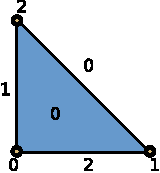
\includegraphics[width=\smallfig]{chapters/kirby-2/pdf/reftri.pdf}
  \caption{The reference triangle, with vertices, edges, and the
    face numbered.}
  \label{fig:reftri}
\end{figure}

\begin{figure}
\bwfig
 \centering
  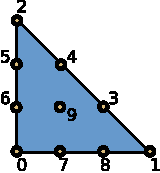
\includegraphics[width=\smallfig]{chapters/kirby-2/pdf/P3.pdf}
  \caption{The cubic Lagrange triangle, with nodes in the dual basis
    labelled. Note that the labels in this figure correspond to the
    FIAT reference element numbering which is different from the
    numbering imposed by the UFC ordering convention explained in
    Chapter~\ref{chap:alnes-2}.}
  \label{fig:p3}
\end{figure}

For this example, the graded incidence relation is stored as
\begin{verbatim}
{ 0: { 0: [ 0 ] ,
       1: [ 1 ] ,
       2: [ 2 ] } ,
  1: { 0: [ 3 , 4 ] ,
       1: [ 5 , 6 ] ,
       2: [ 7 , 8 ] } ,
  2: { 0: [ 9 ] } }
\end{verbatim}

\section{Functional evaluation}

In order to construct nodal interpolants or strongly enforce boundary
conditions, FIAT also provides information to numerically evaluate
linear functionals.  These rules are typically exact for a certain
degree polynomial and only approximate on general functions.  For scalar
functions, these rules may be represented by a collection of points and
corresponding weights $\{ x_i \} , \{ w_i \}$ so that
\begin{equation}
\ell( f ) \approx w_i f(x_i).
\end{equation}

For example, pointwise evaluation at a point \( x \) is simply represented
by the coordinates of \( x \) together with a weight of one. If the
functional is an integral moment, such as
\begin{equation}
\ell( f ) = \int_T g f \dx,
\end{equation}
then the points $\{ x_i \}$ will be those of some quadrature rule and
the weights will be $w_i = \omega_i g(x_i)$, where the $\omega_i$
are the quadrature weights.

This framework is extended to support vector- and tensor-valued function
spaces, by including a component corresponding to each point and weight.
If \( v \) is a vector-valued function and \( v_\alpha \) is its
component, then functionals are written in the form
\begin{equation}
\ell( v ) \approx w_i v_{\alpha_i}(x_i),
\end{equation}
so that the sets of weights, components, and points must be conveyed to
the client.

This framework may also support derivative-based degrees of freedom
by including a multi-index at each point corresponding to a particular
partial derivative.

\section{Overview of fundamental class structure}

Many FEniCS users will never directly use FIAT; for them, interaction
will be moderated through a form compiler such as FFC.
Others will want to use the FIAT basis functions in other contexts.
At a basic level, a user will access FIAT through top-level classes
such as \( \texttt{Lagrange} \) and \( \texttt{RaviartThomas} \) that
implement the elements.  Typically, the class constructors accept the
reference element and order of function space as arguments. This gives
an interface that is parametrized by dimension and degree. The classes
such as \texttt{Lagrange} derive from a base class \texttt{FiniteElement}
that provides access to the three components of the Ciarlet triple.

The function space \( P \) is modelled by the base class
\texttt{PolynomialSet}, which contains a rule for constructing the base
polynomials \( \phi_i \) (e.g. the Dubiner basis) and a multidimensional
array of expansion coefficients for the basis of \( P \).  Special
subclasses of this provide (possibly array-valued) orthogonal bases as
well as the rules for constructing supplemented and constrained bases.
These classes provide mechanisms for tabulating and differentiating
the polynomials at input points as well as basic queries such as the
dimension of the space.

The set of finite element nodes is similarly modeled by a class
\texttt{DualBasis}.  This provides the functionals of the dual basis as
well as their connection to the reference element facets.  The functionals
are modeled by a \texttt{FunctionalSet} object, which is a collection of
\texttt{Functional} objects.  Each \texttt{Functional} object contains a
reference to the \texttt{PolynomialSet} over which it is defined and the
array of coefficients representing it and owns a \texttt{FunctionalType}
class providing the information described in the previous section.
The \texttt{FunctionalSet} class batches these coefficients together in
a single large array.

The constructor for the \texttt{FiniteElement} class takes
a \texttt{PolynomialSet} modeling the starting basis and a
\texttt{DualBasis} defined over this basis and constructs a new
\texttt{PolynomialSet} by building and inverting the generalized
Vandermonde matrix.

Beyond this basic finite element structure, FIAT provides quadrature such
as Gauss-Jacobi rules in one dimension and collapsed-coordinate rules in
higher dimensions.  It also provides routines for constructing lattices
of points on each of the reference element shapes and their facets.

In the future, FIAT will include the developments discussed already
(more general reference element geometry/topology and automatic
differentiation).  Automatic differentiation will make it easier
to construct finite elements with derivative-type degrees
of freedom such as Hermite, Morley, and Argyris.  Additionally,
we hope to expand the collection of quadrature rules and provide
more advanced point distributions, such as Warburton's warp-blend
points~\citep{Warburton2005}.

Finally, we may group the classes used in FIAT into several kinds,
and the relationship between these kinds of classes is expressed in
Figure~\ref{fig:struct}.  Top-level classes implement particular finite
elements, such as Lagrange or Raviart--Thomas.  These depend on classes
that implement the underlying reference shapes, polynomial sets, and
dual bases. The polynomial sets are linear combinations of orthogonal
expansions. Sometimes those linear combinations are constructed via
projection (requiring quadrature) or null spaces of linear functionals.
Dual bases are collections of linear functionals that can act on a
polynomial set over some domain.

\begin{figure}
  \centering
  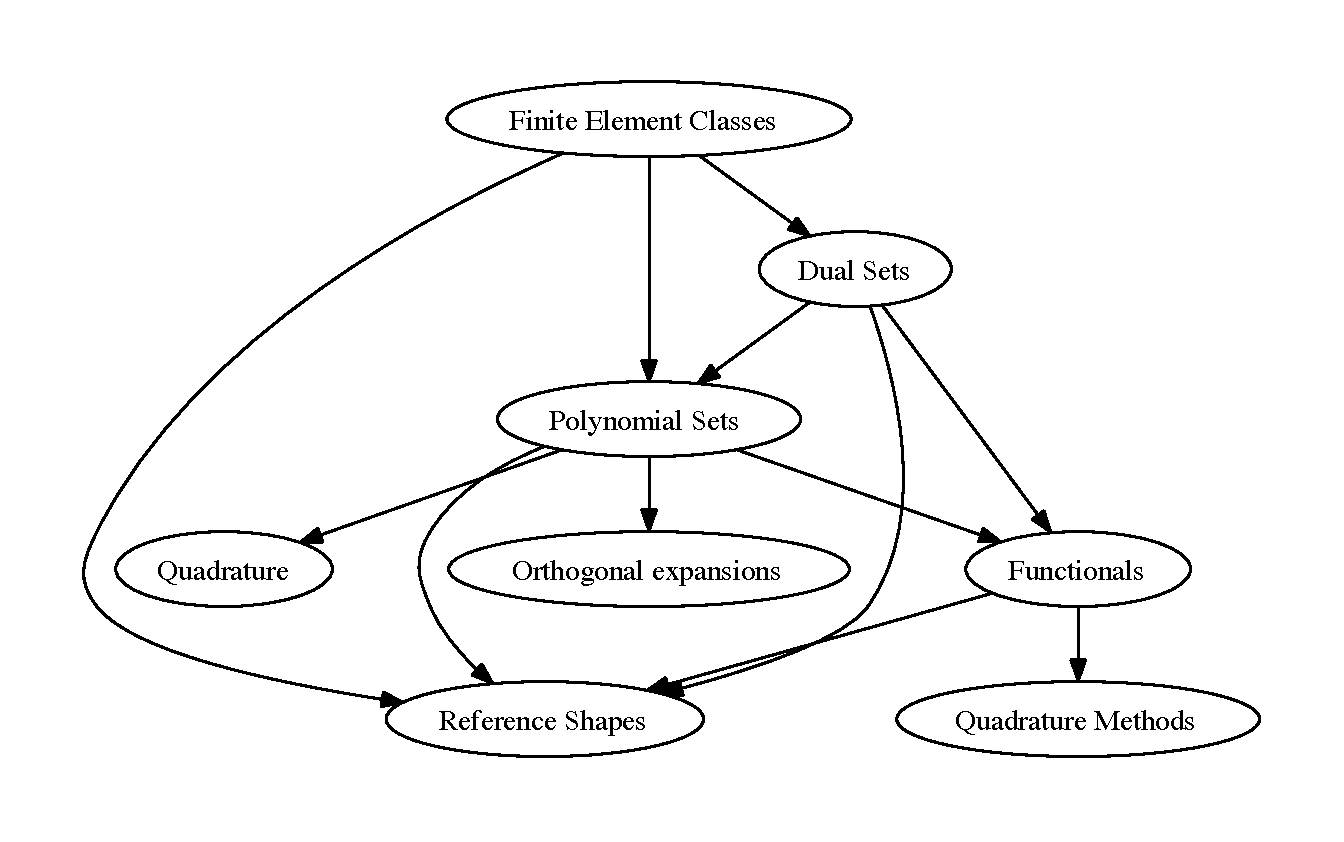
\includegraphics[width=\largefig]{chapters/kirby-2/pdf/struct.pdf}
  \caption{General relationship between the kinds of classes in FIAT.}
  \label{fig:struct}
\end{figure}
